\chapter{Solving Einstein Equations}

While studying gravitational collapse of a scalar field we got a set of differential equations. These differential equations were complicated enough that any effort to find an analytical solution was futile. One can always make some approximations and get some understanding of the solutions, but to get a complete solution we need to use numerical techniques. In this chapter we will discuss about how to solve differential equations on a computer.




\section{Finite difference methods}

Solving differential equations is required in almost every field of Science and although analytical solution are the best thing one can get, they are hard to come by.
Most of the time we have to resort to solving differential equation numerically. There a lot of methods out there developed to solve differential equations, each of them have their own advantages and dis-advantages. In our case we will be using a class of methods called finite difference methods.

\index{Finite difference methods} Finite difference methods are the most intuitive and easy to implement methods. They are derived using the taylor series and give a discrete approximation of the strong from of the differential equations.

To get some intuition about finite difference methods let us start with a very simple example. These simple examples will demonstrate some of the most important concepts of finite difference computing.

Suppose that we want to find the value of the derivative of the function $f(x) = x^3$ at $x =1$. We know that the answer should be $3$. But, let us say that we do not know the exact formula and want to approximate the derivative.
The simplest way to do this would be using the formula of the derivative itself,

\begin{equation}
    \frac{dy(x_0)}{dx} = \lim_{h \to 0}\frac{y(x_0 + h) - y(x_0)}{h}
\end{equation}

The definition of derivative gives us the exact answer in the limit. What we can do is to take $h$ to a small non-zero number and see if that gives us an approximate answer.

\begin{equation}
    \frac{dy(x_0)}{dx} \approx \frac{y(x_0 + h) - y(x_0)}{h} , \text{for } h << 1
\end{equation}\label{eq:first_order}

We have shown the results of using the equation \ref{eq:first_order} to approximate the derivative of $x^3$ at $x=1$ in the figure \ref{fig:x^3_error_order1}. Y axis in the figure is the log error of the approximation and X axis is the log of the \index{step size} step size ($h$). Figure \ref{fig:x^3_error_order1} has a lot of stuff going on in it and we will break it down into parts. There are three line in the figure, each line represents calculations done at different sized floats. Before we move on we will briefly look at how computers store decimal numbers.

\subsection{Floating point arithmetic}

\index{Floats} Floats are how computers internally represent decimal numbers. A larger sized float can handel both a larger number and more significant digits\index{significant digits}. Because computers can only stores a fixed number of digits after the decimal point we get \index{floating point errors} floating point errors whenever any calculation is done on these floats. For example we know that $\frac{1}{3}$ has a recurring decimal expansion, but if we want to save $\frac{1}{3}$ in the computer, in its decimal representation, then there will be a small error because we can only store a fixed number of significant digits.


Table \ref{table:floats} has the information about different kind of floats used in the graphs. \index{Precision}Precision denotes the number of significant digits that a particular type of float can store, for example, float32 can store just 6 numbers after the decimal point which is why $\frac{1}{3}$ is stored as $0.33333334$. Also, note that the there is a huge difference in the largest number that can be stored between different kind of floats. If we try to store a number larger than the maximum number that a float type can hold we get an overflow error and computer starts giving us random garbage. Different languages and libraries deal with such errors in different ways and it is not worth going into the specifics, but the bottom line is that we can not work with float64 if our systems have numbers larger than $1.79*10^{308}$.


Most of the modern computers chips use float64 internally and they have CPU circuits that are very efficient in working with float64 numbers. Float64 denotes that this number will use 64bits of memory, while float32 numbers only use 32bits of memory; this means that we can store more float64 numbers in the same amount of memory. What this means in practical terms is that a we can store around $10^9$ floats in $8GB$ of RAM, or a matrix with approximately 31000 rows and columns. If we are not clever with what we are storing in our RAM there is real danger that we may run out of memory, which will cause an error and our program will stop.


Among the parameters listed in Table \ref{table:floats} the most important parameter for any calculation is the precision. As already mentioned whenever we perform any kind of operation on a floating point number there is an error due to the \index{finite precision}finite precision of floating point numbers.
We can see this phenomenon quite easily just by adding $1.0$ to $\frac{1}{3}$ stored as a float32. If we add $1.0$ to $0.\overline{33}$, $10000$ times the expected answer is $10000.\overline{33}$ which in float32 precision should be $10000.3333334$. But, we see that the actual answer that we get is $10000.334$, that is we have lost 4 significant digits.
This loss of accuracy is what we call \index{floating point error}floating point error and this is the reason why using float32 for numerical computations is a bad idea. If we use float64 instead of float32 we will still lose 4 significant digits but it will not so much because we will still have 11 significant digits in the decimal to work with. We should mention here that there is no hard and fast formula for how many digits will we lose per operation and it depends on the language and libraries used as many of them are optimized to reduce floating point errors.


We will discuss one final point before we wrap up this section and go back to developing finite difference algorithms.





\begin{table}
    \centering
    \begin{tabular}{||m{2cm} | m{3.2cm} | m{1.5cm} | m{4.5cm}||}
        \hline
        Float type & Largest Number that can be stored* & Precision & How is $\frac{1}{3}$ internally stored \\ [0.5ex]
        \hline\hline

        Float32    & 3.40e+38                           & 6         & 0.33333334                             \\

        Float64    & 1.79e+308                          & 15        & 0.3333333333333333                     \\

        Float128   & 3.36e+4932                         & 18        & 0.33333333333333333334                 \\ [1ex]
        \hline
    \end{tabular}
    \caption{This table shows the largest number that can be represented by a particular type of float (* rounded off to two decimal places). Precision denotes the number of significant decimal digits that can be represented by a float type.}
    \label{table:floats}
\end{table}



\begin{figure}[hbt!]
    \centering
    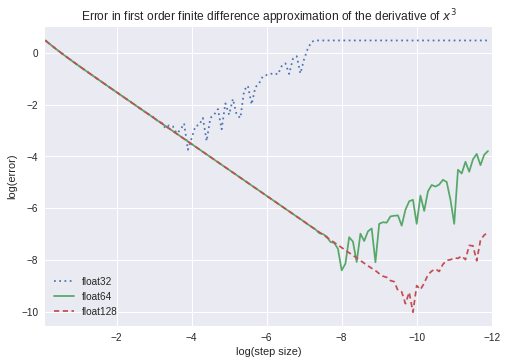
\includegraphics[width=\textwidth]{images/x^3_error_order1.png}
    \caption{This plot show error of using finite difference to approximate the derivative of $x^3$ vs the step size. Observe that the error falls almost linearly until we reach the step sizes smaller than $10^{-8}$ after which it starts to grow due to floating point errors. Also, observe that for reasonable step sizes the error falls with a slope of 1, which is why such approximations are called first order. }\label{fig:x^3_error_order1}
    \index{figures}
\end{figure}

\begin{figure}[hbt!]
    \centering
    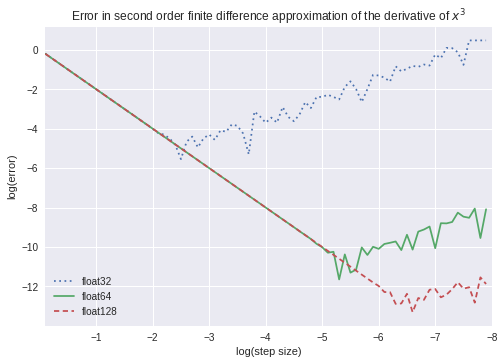
\includegraphics[width=\textwidth]{images/x^3_error_order2.png}
    \caption{This plot show error of using finite difference to approximate the derivative of $x^3$ vs the step size. Observe that the error falls almost linearly until we reach the step sizes smaller than $10^{-10}$ after which it starts to grow due to floating point errors. Also, observe that for reasonable step sizes the error falls along a line with slope 2 which is to be expected of a second order approximation. }\label{fig:x^3_error_order2}
    \index{figures}
\end{figure}

\begin{figure}[hbt!]
    \centering
    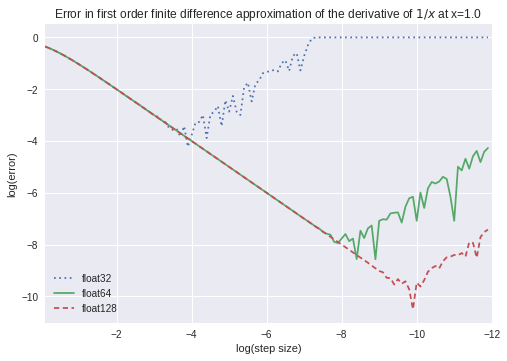
\includegraphics[width=\textwidth]{images/1_x_error_at_1.png}
    \caption{This plot show error of using finite difference to approximate the derivative of $\frac{1}{x}$ vs the step size.}\label{fig:1/x_1}
    \index{figures}
\end{figure}

\begin{figure}[hbt!]
    \centering
    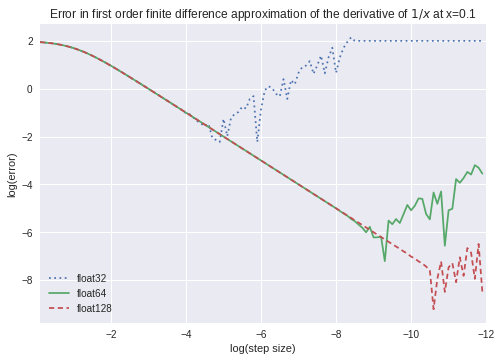
\includegraphics[width=\textwidth]{images/1_x_error_at_p1.png}
    \caption{This plot show error of using finite difference to approximate the derivative of $\frac{1}{x}$ vs the step size.}\label{fig:1/x_0.1}
    \index{figures}
\end{figure}


\begin{figure}[hbt!]
    \centering
    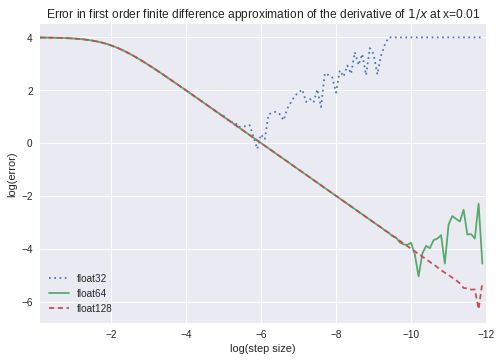
\includegraphics[width=\textwidth]{images/1_x_error_at_p01.png}
    \caption{This plot show error of using finite difference to approximate the derivative of $\frac{1}{x}$ vs the step size.}\label{fig:1/x_0.01}
    \index{figures}
\end{figure}